\documentclass[11pt,letterpaper]{article}
\usepackage[margin=.83in,top=.75in,bottom=.79in,headheight=15pt,headsep=13pt]{geometry}
\usepackage{amsmath,amssymb,booktabs,array,xcolor,tikz,hyperref,fancyhdr}
\usetikzlibrary{arrows.meta}
\definecolor{navy}{HTML}{153449}\definecolor{teal}{HTML}{116556}
\definecolor{ink}{HTML}{334F60}\definecolor{wash}{HTML}{EAF4F1}\definecolor{copper}{HTML}{934925}
\hypersetup{colorlinks=true,linkcolor=teal,urlcolor=teal,pdftitle={SAT in the digits of a three-lane routing count},pdfauthor={Research note prepared for Dominic Dabish}}
\pagestyle{fancy}\fancyhf{}\fancyhead[L]{\small\sffamily\color{teal}PERMUTATION PROGRAMS}\fancyhead[R]{\small\sffamily\color{ink}DECISION AND COUNTING}
\fancyfoot[L]{\footnotesize\sffamily\color{ink}Working manuscript for Dominic Dabish \enspace / \enspace 21 November 2026}\fancyfoot[R]{\small\sffamily\color{navy}\thepage}
\renewcommand{\headrulewidth}{.35pt}\setlength{\parindent}{0pt}\setlength{\parskip}{4.9pt}\setlength{\emergencystretch}{1.4em}
\setlength{\abovedisplayskip}{5pt}\setlength{\belowdisplayskip}{5pt}
\newcommand{\pg}[2]{\newpage\phantomsection\pdfbookmark[1]{#1}{#2}{\LARGE\bfseries\color{navy}#1\par}\vspace{3pt}}
\newcommand{\subh}[1]{\par\smallskip{\large\bfseries\color{teal}#1}\par\nobreak}
\newcommand{\lab}[1]{\textbf{\color{navy}#1}\enspace}
\newcommand{\boxit}[1]{\par\smallskip\colorbox{wash}{\parbox{\dimexpr\linewidth-2\fboxsep\relax}{\vspace{3pt}#1\vspace{3pt}}}\par\smallskip}
\newcommand{\FF}{\mathbb F}\newcommand{\sat}{\mathop{\#\mathrm{SAT}}}\newcommand{\id}{\mathrm{id}}\newcommand{\pf}{\operatorname{Pf}}
\newcommand{\win}{\mathop{\mathrm{win}}}\newcommand{\bit}{\operatorname{bit}}\newcommand{\supp}{\operatorname{supp}}
\newcommand{\source}[2]{\href{#1}{#2}}
\begin{document}
\phantomsection\pdfbookmark[1]{The classification}{cover}
{\sffamily\small\color{ink}RESEARCH NOTE \hfill COMPUTATIONAL COMPLEXITY}\par
\vspace{8pt}
{\fontsize{26}{30}\selectfont\bfseries\color{navy}SAT in the digits of a\\three-lane routing count\par}
\medskip
Line up three labeled wires. Each switch can exchange two of them, either unconditionally or when a named Boolean control takes a specified value. Use the same setting wherever that name occurs. Close the outputs back onto the inputs. A setting wins when following the wires makes a single tour through all lanes. Let $W(P)$ count the winning settings of program $P$.

\boxit{\textbf{Main reduction.} For every Boolean CNF $F$ and positive precision $b$, construct one three-lane program $P$ in polynomial time in $|F|+b$ (with variables explicitly counted). Each control appears at most three times, and
\[
                         W(P)\equiv\sat(F)\pmod {2^b}.
\]
The construction can make the all-zero setting win and put the winning fraction within $1/(3\cdot 2^k)$ of $1/3$, for any requested even $k\ge2$.}

\subh{What changes when a control gets a third switch}
\begin{center}
\renewcommand{\arraystretch}{1.22}
\begin{tabular}{@{}p{.32\linewidth}p{.27\linewidth}p{.32\linewidth}@{}}
\toprule
Question on three lanes & At most two uses & At most three uses\\\midrule
Find one winning setting & Polynomial time & Polynomial time\\
Count modulo $2^b$, fixed $b$ & Polynomial time & Preserves $\sat\bmod 2^b$\\
Count modulo $3^a$, fixed $a$ & Polynomial time & Polynomial time\\
Estimate $W$ to relative error & FPRAS & FPRAS\\
Compute $W$ exactly & \#P-complete$^*$ & \#P-complete$^*$\\\bottomrule
\end{tabular}
\end{center}
{\small $^*$For polynomial-time counting reductions. The three-use construction recovers a whole input count from a single residue. An FPRAS is a randomized relative approximation scheme running in time polynomial in input size and inverse relative error.}

Two programs of 56 switches illustrate the distinction. Encoding $(x)\land(x)$ at one bit yields 343 winning settings out of 1,024. Encoding $(x)\land(\neg x)$ yields 340 out of 1,024. Turning on only control 10 gives a tour in both. Their units digits recover the counts of models modulo two. Page 9 constructs a specified higher digit that decides satisfiability for arbitrary inputs.

The four-lane extension on page 6 preserves the two-use binary algorithm. The width bound on page 4 explains why adding any fixed number of lanes with bounded reuse preserves polynomial-time existence. P versus NP remains open. The proofs here are working derivations. Priority for their combined statements has not been established.

\pg{How this route fits the evidence}{history}
\begin{center}
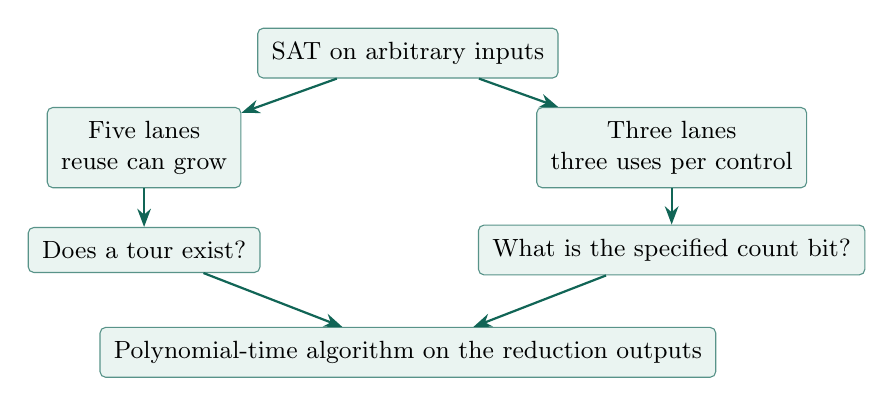
\begin{tikzpicture}[>=Stealth,box/.style={draw=teal!70,fill=wash,rounded corners=2pt,inner sep=5pt,align=center,font=\small},a/.style={->,thick,teal}]
\node[box] (sat) at (0,2.15) {SAT on arbitrary inputs};
\node[box] (five) at (-3.35,.95) {Five lanes\\reuse can grow};
\node[box] (three) at (3.35,.95) {Three lanes\\three uses per control};
\node[box] (exists) at (-3.35,-.35) {Does a tour exist?};
\node[box] (digit) at (3.35,-.35) {What is the specified count bit?};
\node[box] (goal) at (0,-1.65) {Polynomial-time algorithm on the reduction outputs};
\draw[a] (sat)--(five);\draw[a] (sat)--(three);\draw[a] (five)--(exists);\draw[a] (three)--(digit);
\draw[a] (exists)--(goal);\draw[a] (digit)--(goal);
\end{tikzpicture}
\end{center}
Either bottom input problem, if solved in deterministic polynomial time on all outputs of its SAT reduction, gives $\mathrm P=\mathrm{NP}$. A proof of $\mathrm P\ne\mathrm{NP}$ must exclude every deterministic polynomial-time SAT algorithm. Lower bounds for a chosen wiring model address a narrower quantifier.

{\small\renewcommand{\arraystretch}{1.28}
\begin{tabular}{@{}p{.16\linewidth}p{.79\linewidth}@{}}
\toprule
Period & Result and its bearing on the route\\\midrule
1971--73 & Cook and Levin's completeness results and Karp's reductions turn one uniform SAT algorithm into algorithms for every problem in NP.\\
1975--79 & Baker, Gill and Solovay give oracles with opposite answers. Valiant establishes the difficulty of exact permanent computation and polynomial algorithms for fixed binary precision. This motivates separating decision, approximation and count digits.\\
1985--94 & Barrington gives a width-three representation by parity and mod-three gates, then a width-five simulation of logarithmic-depth formulas. Cai and Lipton derive a finite-group AND lower bound by thinning occurrences. Pages 3--4 specialize those ideas to switches.\\
1994--2009 & Natural proofs constrain certain constructive, large circuit properties under a pseudorandomness assumption. Algebrization rules out another class of approaches. In a different direction, the AKS primality algorithm is an unconditional example of a difficult-looking decision problem entering P.\\
2011--22 & Williams separates NEXP from polynomial-size ACC circuits. Hirai and Namba give a fixed-power-of-two hafnian algorithm. Idziak and coauthors analyze program satisfiability over finite groups. The circuit and group restrictions matter to the conclusions.\\
\bottomrule
\end{tabular}}
The generalized Sudoku work enters through a direct, counting-preserving encoding. Use one variable per cell--symbol pair and assert exactly one symbol per cell and exactly one copy of each symbol per row, column and region, with the givens fixed. The satisfying assignments are the completions. The same construction on page 8 therefore preserves their low count bits. Standard $9\times9$ boards have fixed size. Asymptotic claims concern growing board families. References and the broader historical map appear on page 11.

\pg{Finding a tour on three lanes}{characters}
Label three lanes by $\FF_3$. Every transposition is a reflection $s_h(z)=-z+h$, where $h$ is the sum of its two exchanged lane labels modulo three. Compose on the right in gate order. After gate $j$ the product acts by $z\mapsto e_jz+u_j$, where $e_j=(-1)^{p_j}$, and $p_j$ is an affine binary form on the input. Initially $e_0=1$ and $u_0=0$. If gate $j$ fires, its sign flips and the translation changes by $e_{j-1}h_j$. Thus
\[
       2u_L=\sum_{j=1}^{L}h_j(e_{j-1}-e_j)\pmod3.
\]
A three-cycle occurs precisely when $p_L=0$ and $u_L\ne0$. The final sign condition gives either an empty set or an affine cube $H$ of dimension $d\in\{n-1,n\}$. On $H$ the displayed sum is an integer polynomial $F$ in the sign characters $\chi_S(x)=(-1)^{\sum_{i\in S}x_i}$. Combine equal masks. There are at most $L+1$ masks because each prefix supplies just one.

\subh{A deterministic witness and a density bound}
The characters on $H$ are linearly independent over $\FF_3$. Their dot products vanish for distinct masks and each self-product sums to $2^d$, a unit. Drop the zero coefficients modulo three, leaving $s$ characters. If $s=0$, every even output fixes all three lanes. Otherwise one of the two restrictions of each free input bit keeps a nonzero character expansion. Fix that bit accordingly and continue to obtain an actual winning setting.

Every translate of $F\bmod3$ lies in the span of the same $s$ characters. Choose a basis of translates. Their supports cover $H$, since at every point some translate is nonzero. All translates have equal support size, so $|\supp F|\ge 2^d/s$. On the full cube, a nonempty winning set has density at least $1/(2s)$. Checking emptiness exactly and sampling $O(s\varepsilon^{-2}\log(1/\delta))$ uniform inputs gives relative error $\varepsilon$ with failure probability at most $\delta$, for $0<\varepsilon,\delta<1$.

\subh{Counting modulo powers of three}
For fixed $a\ge1$ put $h=\lceil a/2\rceil$, $D=h+a-1$ and
\[
 B(y)=\sum_{j=h}^D {D\choose j}y^j(1-y)^{D-j}.
\]
Use the integer lift of $F$ above. If $3\mid F$, each term of $B(F^2)$ is divisible by $3^a$. Otherwise $F^2\equiv1\pmod3$ and each omitted binomial term with $j<h$ is divisible by $3^a$. Hence $B(F^2)$ is the winning indicator modulo $3^a$ on $H$. Multiply sparse expressions using $\chi_S\chi_T=\chi_{S\triangle T}$. Summing them over $H$ retains only $2^d$ times the constant coefficient. This gives $L^{O(a)}\operatorname{poly}(n,a)$ bit time, interpreting $L$ as at least two. The proof allows any number of uses of any input bit.

\pg{A width bound for bounded reuse}{width}
\boxit{\textbf{Sparse-witness bound.} Fix $r\ge1$. For a program on $w\ge2$ lanes using each of $n$ controls at most $r$ times, every attainable output permutation can be attained within $O_r(w^{2r})$ bit flips of \emph{any} initial setting. Enumerating that ball gives time $(n+2)^{O_r(w^{2r})}\operatorname{poly}(w,L)$.}

Pick a nearest setting yielding the target permutation. Call its differences from the initial setting active controls. For each use of an active control, conjugate its transposition by the product of all preceding gates at the target setting. Flipping any chosen active controls back multiplies the original output on the left by the ordered product of their conjugated occurrences. To see this, move each change leftward across the original prefix in the product. Every conjugate is again a single transposition.

The type of a control is its ordered list of these conjugates. There are at most $T=\sum_{j=1}^{r}\binom{w}{2}^{j}$ types. Fix one type with $s\le r$ occurrences. The subgroup generated by its transpositions acts within the connected components of a graph with at most $r$ edges. Each component has at most $r+1$ vertices. Every group element therefore has order dividing $e=\operatorname{lcm}(1,\ldots,r+1)$.

\lab{Thinning the occurrences.} Put $N_0=e$ and $N_{i+1}=(rN_i)^2$. Suppose $N_{2r}$ or more active controls have the same type. Start with their common $s$ ranks in a single time interval. In any segment with at least two ranks per control, draw an interval from its first to last rank for each remaining control. With $M$ controls there are either at least $\sqrt M$ disjoint intervals or at least $\sqrt M$ sharing a point. For the latter alternative, greedily pierce at the earliest right endpoint and remove the intervals pierced. The chosen endpoints come from disjoint intervals and together meet every interval.

In the disjoint case keep the disjoint family and finish this segment. In the common-point case a cut between gate positions lies inside all selected intervals, since every occurrence time is distinct. Retain those with the most frequent number of ranks to the left and split at the cut. At least $\sqrt M/r$ controls survive. Apply the same procedure to both children, carrying the common surviving family forward. Single-rank segments finish immediately. Each split partitions ranks into two nonempty sets, so at most $2r-1$ segments are processed. Later thinning preserves the conclusions for finished segments.

Choose exactly $e$ survivors. In each finished segment their combined word is $e$ copies of one fixed subword in some order of controls. Its product is identity. Deleting all $e$ controls preserves the target and contradicts minimality. Thus at most $(N_{2r}-1)T$ flips suffice. The constants give an existence theorem and can be extremely large.

\lab{Consequences.} Any direct representation of $n$-bit AND by this acceptance predicate with $r=3$ requires $w=\Omega(n^{1/6})$, even if the other controls can be chosen freely, since attaining acceptance requires turning on all $n$ named inputs. Under the Exponential Time Hypothesis for 3-SAT, a polynomial-size existence reduction on every $n$-variable 3-CNF cannot have $w=o((n/\log n)^{1/6})$ at three uses. Otherwise enumerating the ball decides 3-SAT in $2^{o(n)}$ time after removing duplicate clauses. This width bound concerns individual swaps. Cai--Lipton's fixed-group AND bound is a close antecedent [5].

\pg{Two uses give a matching algorithm}{matching}
\lab{Step 1. Prefix signs become edges.} For a three-lane program put $q_j=p_j\in\{0,1\}$, with $q_0=q_L=0$ for even output. The swap at $j$ fires exactly when $z_j=q_{j-1}\oplus q_j$. A fixed gate imposes $z_j=1$. Two occurrences of one control impose $z_i\oplus z_j=0$ or $1$, according to their literal signs. A singleton imposes no equation. These prefix strings are in bijection with the even settings of all occurring controls. Writing the translation from page 3 gives
\[
                      u_L=\sum_{j=1}^{L-1}(h_j-h_{j+1})q_j\pmod3.
\]
Each free $q_j$ occurs in at most two parity equations, since only its two neighboring gates can mention it. Cancel repeated appearances in one equation. Make a vertex for each equation and an edge for each column with two remaining ones. Join one-occurrence columns to a dummy vertex with demand equal to the XOR of all original demands. Zero columns contribute independent factors $1+z^{h_j-h_{j+1}}$. A selected edge has weight $z^{h_j-h_{j+1}}$ in $R=(\mathbb Z/2^b)[z]/(z^3-1)$. We need the sum of the coefficients of $z,z^2$ in the weighted parity subgraphs.

\lab{Step 2. Unique completions to ordinary matchings.} Split any high-degree parity vertex into degree-at-most-three vertices joined by a tree. Give one vertex its original demand and the others zero. The internal selection is determined by leaf elimination. At each vertex give each incident edge a separate port. Selecting an external edge covers its two ports. Add these internal edges to give exactly one completion for each permissible set of covered ports.
\begin{center}\small\renewcommand{\arraystretch}{1.15}
\begin{tabular}{@{}lll@{}}\toprule
Ports & Even demand & Odd demand\\\midrule
1 & Port joined to a private vertex & Lone port\\
2 & Join the two ports & One private vertex joined to both\\
3 & Private center joined to all, plus one port pair & Triangle on the ports\\\bottomrule
\end{tabular}\end{center}
Zero ports require even demand. The three-port even case works because zero selected ports allow one matching using the port-pair edge and two selected ports leave one port for the center. Each allowed external selection has multiplicity one.

\lab{Step 3. Remove matching signs at fixed precision.} In vertex order, a Pfaffian counts each perfect matching $M$ with sign $(-1)^{c(M)}$, where $c(M)$ is the number of crossing pairs of edges in that order. Multiply each signed term by $(1-2)^{c(M)}$. Modulo $2^b$ it suffices to enumerate sets of up to $b-1$ crossing pairs. Force their union of edges, skip conflicting endpoints, and compute the remaining signed sum with a Pfaffian minor, including the cofactor sign. Crossing pairs may share the same forced edge. This is polynomial for fixed $b$ and gives the unsigned matching count. Hirai--Namba [6] give a polynomial hafnian algorithm for this precision. The reference code uses integer Pfaffians with balanced-base encoding of polynomial weights, then folds degrees modulo three. A base exceeding twice the number of possible matchings prevents carries since each coefficient is a signed matching count.

\pg{A fourth lane still permits fixed binary precision}{four}
Identify four points with $V=\FF_2^2$. Their full permutation group is the affine group $V\rtimes\mathrm{GL}(2,2)$, since there are $4\cdot6=24$ different affine bijections. Every individual transposition has a nonidentity order-two linear part $A$ that permutes the three nonzero vectors as a transposition. Its translation $d$ is its value at the zero vector. Thus the sequence of linear parts, with the original control keys, is itself a three-lane switch program.

If the final linear part $T$ is even on the three nonzero vectors, the affine output is even on four lanes and cannot be a four-cycle. Translations are even, and the embedded linear group fixes zero. If $T$ is odd, it fixes a line and $I+T$ has rank one and kernel that line. Let $\ell_T(v)$ be its binary nonzero test. It is a linear functional. An affine output $v\mapsto Tv+u$ squares to translation by $(I+T)u$. An odd output is a four-cycle precisely when $\ell_T(u)=1$.

Putting $Q_{j-1}$ for the prefix linear product and $z_j$ for the gate's actual firing bit gives, for each of the three possible odd $T$,
\[
             \ell_T(u)=\bigoplus_{j=1}^L d'_j,\qquad
             d'_j=z_j\,\ell_T(Q_{j-1}d_j).
\]
Over the integers, the XOR of bits is $\sum_{k\ge1}(-2)^{k-1}\sum_{|J|=k}\prod_{j\in J}d'_j$. Reduce modulo $2^b$ and retain $k\le b$. For each set of marked gates, require their controls to fire, fix the corresponding named bits everywhere, and discard inconsistent requirements. Enumerate the possible prefix matrices at the marked positions satisfying the displayed tests, and impose final matrix $T$. There are at most $6^b$ prefix tuples. Knowing two successive prefix values fixes the product on the intervening segment. All segments are disjoint in time, so no additional occurrence of a control is created.

\subh{Counting simultaneous segment values}
In each segment reset its local $q_0=0$ and prescribe final sign $q_L\in\{0,1\}$ from the required matrix. The equations on page 5 still have at most two occurrences per free column, including when a control spans two segments. Each segment contributes its own modulo-three translation coordinate. The displayed translation on page 5 gains the constant $h_Lq_L$ in that segment. An empty segment must have identity target. Let $s\le b+1$ be the number of segments and $v\in\FF_3^s$ the desired vector after subtracting the constants.

For a direction $a$, project weights to $a\cdot u$ and use the same one-coordinate matching algorithm. Let $H_a$ count solutions with $a\cdot u=a\cdot v$ and $D$ count all solutions to the sign equations. Select one direction from each pair $\{a,-a\}$ with $a\ne0$. The desired count is
\[
        3^{-s}\left[D+\sum_{\{a,-a\}}(3H_a-D)\right]\pmod{2^b}.
\]
For one fixed $u$, the bracket contributes $3^s$ if $u=v$ and zero otherwise, by counting directions orthogonal to $u-v$. Three is invertible modulo $2^b$. Summing the marked sets gives a deterministic $L^{O(b)}\operatorname{poly}(n)$ algorithm with constants depending on $b$. Appending a fourth lane and a fixed swap attaching it to an old lane preserves the number of cycles of every three-lane setting. The three-use hardness on page 8 transfers as well.

\pg{Why exact counting is already hard at two uses}{exact}
Given a connected loopless graph $G$ on an even number $v$ of vertices and with $m$ edges, let $a_j$ count the $j$-edge subsets with odd degree at every vertex. Since their total degree is $2j$, $a_{v/2}$ counts perfect matchings. We describe one exact routing-count query that recovers this coefficient. Counting bipartite perfect matchings is the zero--one permanent [3]. Disconnected inputs can be handled component by component, and odd components have zero perfect matchings.

\lab{Encode an odd subgraph.} Replace each edge by $\lambda=12(m+1)$ parallel copies and take an Euler tour. Write its $m\lambda+1$ consecutive vertex visits, keeping distinct first and last visits to its root. At each vertex join its visits by a path on those time slots. Give each path edge its own bit controlling a reflection $R(z)=-z$ at each endpoint. Add one fixed $R$ at one visit to each vertex. Between consecutive visits insert the fixed rotation $C(z)=z+1$. Append $C^{-m\lambda}$. Each bit controls two individual transpositions.

On the actual tour edges let $q_e$ be the running parity of the reflections fired. Give the virtual edges immediately before and after the walk parity zero. The final parity is indeed even since there are $v$ fixed reflections and every control occurs twice. The change at each visit is the XOR of the two adjacent edge parities. At a given vertex the XOR of these changes is one. Conversely any odd-degree subset of tour edges can supply the $q_e$. At each vertex the demands after removing the fixed reflection have even total, and the incidence equations on its visit path have a unique bit solution. Therefore settings and odd subgraphs of the expanded multigraph are in bijection. The inserted rotations yield translation $\sum_e(-1)^{q_e}-m\lambda\equiv\sum_e q_e\pmod3$. There are $D=2^{m\lambda-v+1}$ settings.

\lab{Recover the minimum-degree coefficient.} Let $h_r$ count settings of translation $r$ and evaluate $Z=h_0+h_1\omega+h_2\omega^2$ at a primitive cube root of unity. A bundle of parallel edges contributes its even or odd choice sum,
\[
 A=\tfrac{(1+\omega)^\lambda+(1-\omega)^\lambda}{2}=\tfrac{1+B}{2},\qquad
 E=\tfrac{(1+\omega)^\lambda-(1-\omega)^\lambda}{2}=\tfrac{1-B}{2},\quad B=3^{\lambda/2}.
\]
These equalities use $1+\omega=e^{i\pi/3}$ and $1-\omega=\sqrt3e^{-i\pi/6}$. Consequently $Z$ is real, $h_1=h_2$, and $Z=D-3W/2$. The oracle gives the signed-base evaluation
\[
        2^m Z=Q(B),\qquad Q(X)=\sum_{j=0}^m a_j(1+X)^{m-j}(1-X)^j.
\]
Each coefficient of $Q$ has absolute value at most $4^m<B/2$. Recover all coefficients by balanced division by $B$. Invert the substitution to recover
\[
              \sum_j a_jY^j=2^{-m}(1+Y)^m Q\!\left(\frac{1-Y}{1+Y}\right).
\]
All integers have polynomial bit length. This proves \#P-hardness under polynomial-time counting reductions. Membership in \#P follows by guessing a control setting and tracing it. For $K_{3,3}$ the actual encoding has 4,316 gates and 1,075 controls. Direct dynamic programming on these gates followed by this decoder gives exactly six perfect matchings.

\pg{Three uses preserve every requested SAT residue}{hard}
\lab{Encode the satisfied clauses.} Make a parsimonious 3-CNF presentation of the input. For example, replace the first two literals of a long clause by a fresh variable $t$ and enforce $t\leftrightarrow(\ell_1\lor\ell_2)$ by three short clauses. Remove tautological clauses but retain all named input variables. Append one fresh clause $(a\lor b)$ on two new variables. This triples the model count and ensures at least one clause. Let $m$ be the new number of clauses and $b_0\ge1$ the requested binary precision.

For each clause $j$, introduce $b_0$ independent bits $y_{ji}$. A constant-length three-lane word realizes $C^{y_{ji}\mathbf1_{\text{clause }j}}$. Indeed this exponent, as a function of at most four bits, is a sum over $\FF_3$ of sign characters (page 3). To implement each term with coefficient $a$, conjugate the fixed $C^a$ by $R$ raised to the parity of its mask. Each parity is a sequence of controlled $R$'s, and $RCR=C^{-1}$. Concatenating the words adds the exponents. Bits unused in the word can be retained by inserting two identical controlled reflections. For a fixed unsatisfying assignment at least $b_0$ ignored selectors make its entire distribution zero modulo $2^{b_0}$. Each satisfying assignment yields the rotation histogram $(1+C)^{mb_0}$.

\lab{Split long-lived controls.} Space the $c>3$ occurrences of a bit over $c-2$ copies in a chain. Each end receives two original occurrences and each interior copy one. Check adjacent copies $p,q$ with a word using one occurrence of each and $b_0$ private bits $z_i$, used twice each. Write $S_k(t)=-t+k$, $R=S_0$, and $U=S_1^{z_1}S_2^{z_2}S_0^{z_3}\cdots$, cycling the subscripts modulo three. The word is
\[
                        U^{-1}R^{1+p+q}UR.
\]
For $p\ne q$ its value is always $R$, with multiplicity $2^{b_0}$. Hence any inconsistent copy assignment contributes zero in the group algebra $(\mathbb Z/2^{b_0})[S_3]$, even when surrounded by other words. If $p=q$, conjugation makes the first factor a reflection. The three multiplicities start at $(1,0,0)$. Conjugating optionally by $S_k$ adds the current vector to its image under the permutation fixing coordinate $k$ and interchanging the others. If two coordinates are equal and the exceptional one differs by $d=\pm1$, choosing $k$ different from the exception moves the exception to $k$ and changes its difference to $-d$. The final $R$ turns reflection $S_j$ into rotation $C^j$. The honest check distribution is
\[
           V=\frac{2^{b_0}-(-1)^{b_0}}3(1+C+C^2)+(-1)^{b_0}C^{b_0\bmod3}.
\]
All copies now have at most three uses. This is an equality check in modular counts. On mismatches the gates still have ordinary settings, whose multiplicity vanishes at the requested precision. That property is what allows both sides of SAT to have winning settings.

\pg{Extracting the answer from a count bit}{bit}
\lab{Normalize the residue.} Work in $(\mathbb Z/2^{b_0})[C]/(C^3-1)$. Set $J=1+C+C^2$, $H=J/3$, and $E=1-H$, using the inverse of three. These last two elements are complementary idempotents. Multiplication by $H$ keeps only total mass times $H$. Since $m\ge1$, $(1+C)^{mb_0}$ has total mass divisible by $2^{b_0}$. Also
\[
                   (1+C)E=-C^2 E,\qquad VE=(-1)^{b_0} C^{b_0\bmod3}E.
\]
Thus every honest satisfying assignment contributes $\pm C^k E$ after all checks. This sign and shift depend only on the word, not its satisfying assignment. One extra optional rotation multiplies by $1+C$ and can reverse the sign on the $E$ component. A fixed rotation shifts the exceptional coordinate to either nonidentity rotation. In the resulting positive $C^kE$ with $k\ne0$, the total weight of the two nonidentity rotations is $1/3$. The fresh clause supplied a multiplicity of three, giving exactly $\sat(F)\bmod2^{b_0}$ in $W$. An optional rotation uses one fresh control twice. For a normalized 3-CNF with $n$ variables and $m$ clauses the construction has $O(n+mb_0^2)$ gates. Its precision parameter is supplied in unary or is polynomial in the source input length.

\subh{Three uses of the reduction}
\lab{Exact recovery.} Choose $b_0=n+1$ for an original $n$-variable formula. The least residue is then the exact number of satisfying assignments, including when all $2^n$ assignments work. This does not equate the full routing count with the input count.

\lab{Every fixed binary digit.} With $b_0=1$, the units digit is $\oplus\mathrm P$-complete. For a fixed higher index $j$, add $j$ independent controls that each trigger two identical consecutive swaps. Every one doubles $W$, moving its units digit to index $j$. For membership, the parity of $\binom W{2^j}$ equals digit $j$, by factoring $(1+x)^W$ over $\FF_2$. A nondeterministic machine guesses $2^j$ distinct winning settings in strictly increasing order. This takes polynomial time for a fixed $j$. The argument distinguishes parity-SAT hardness from the ordinary decision version of SAT.

\lab{A single designated digit for ordinary SAT.} For $n\ge1$ use a selector $s$. When $s=1$ require $F(x)$, and when $s=0$ require at least one of the original $x_i$ to be true. The guarded CNF has $\sat(F)+2^n-1$ models. Compile it with $b_0=n+1$. The bit of $W$ at zero-based index $n$ is one exactly when $F$ is satisfiable. Guarded clauses of length greater than three are split with uniquely determined auxiliaries. This is one deterministic query. Page 10 gives it the same public winning setting on every input. The ordinary existence algorithm on page 3 cannot read the designated bit.

\boxit{\textbf{What would settle equality on this route.} Give a deterministic polynomial-time procedure computing the designated bit on every output of the guarded construction. That would decide SAT. A uniform algorithm for arbitrary specified count bits on the entire two-use family would also suffice, by reconstructing the polynomially many bits of an exact count and applying page 7. The fixed-precision algorithms have exponents depending on precision.}

\pg{Fix the success rate and publish a winning setting}{density}
\boxit{\textbf{Counts close to one third.} Given $F$, $b\ge1$, and an even $k\ge2$, construct one three-lane program on $M$ bits, each used at most three times, for which the all-zero setting wins and
\[
          W\equiv\sat(F)\pmod {2^b},
          \qquad\left|\frac{W}{2^M}-\frac13\right|\le\frac1{3\cdot2^k}.
\]
The construction has polynomial size in $|F|+b+k$. It applies directly to the guarded formula on page 9, so one designated digit decides ordinary SAT under both promises.}

Take the program $P$ of pages 8--9. Ensure that at least one source control must be split. If necessary insert four identical controlled reflections on an already counted variable before splitting. Their product is identity on both values. Every copy of a split control has exactly three controlled transpositions after the checks. Thus the sign on final settings is a nonconstant affine form. Exactly $H=2^{N-1}$ of its $2^N$ settings have even output. There are at least $b$ controls from the selectors on the padded clause, so $N\ge b$.

Append $k$ independent optional rotations and a fixed rotation $C^{-2k}$. Each new control is used twice. The suffix is always even. For even $k$, its exact distribution on rotations is
\[
                     (1+C)^k C^{-2k}=1+\frac{2^k-1}{3}J.
\]
This follows by projecting onto $J/3$ and $1-J/3$ as on page 9, or directly by induction. Set $\alpha=(2^k-1)/3$. Every initial even setting gains $2\alpha$ winning completions, plus one more if that setting already won. An initial odd setting stays odd. Therefore
\[
           W'=W(P)+2\alpha H=W(P)+\alpha 2^N,
           \qquad
           \frac{W'}{2^{N+k}}=\frac13+2^{-k}\left(\frac{W(P)}{2^N}-\frac13\right).
\]
Since $0\le W(P)\le 2^{N-1}$, the deviation bound follows. The additional term in $W'$ is divisible by $2^b$. The new winning fraction is at least $1/4$ on every input. Run the deterministic witness algorithm from page 3 and negate each literal whose named bit is one in the witness. This bijective change of variables preserves all counts and makes the all-zero input win.

\subh{Two examples with very different kinds of verification}
For the two 56-gate examples on page 1, adding $k=40$ optional rotations gives respectively $375{,}299{,}968{,}947{,}543$ and $375{,}299{,}968{,}947{,}540$ winners among $2^{50}$ settings. Exact dynamic programming on the emitted switches gives these integers, including after the all-zero reorientation.

For a decision example where parity by itself is uninformative, use $n=2$. The formula $(x\lor y)\land(\neg x\lor\neg y)$ has two models, while $(x)\land(\neg x)$ has zero. The guarded three-bit outputs have residues $5=101_2$ and $3=011_2$. Both runs use $k=40$ and publish the all-zero winner. The first program has 574 controls and 1,866 gates. The second has 382 controls and 1,218 gates. The residues were obtained by tracing the compiler's filter blocks and applying the exact suffix identity, rather than exhaustively enumerating hundreds of control bits.

\pg{Verification and primary sources}{verification}
\lab{How much can uniform sampling tell us?} For the two equal-size circuits on page 1, the construction on page 10 adds exactly the same integer $2^{10}(2^k-1)/3$ to both counts. They still differ by three. With $M=10+k$ controls the winning probabilities differ by precisely $3/2^M$, while both stay between $1/4$ and $1/2$. Any procedure that observes only independent random win/loss outcomes requires $\Omega(4^M)$ samples to distinguish these two possibilities with constant advantage. Indeed, the one-sample relative entropy of the two Bernoulli laws is $O(4^{-M})$. Relative entropy adds across independent trials and Pinsker's inequality bounds total variation. The input description gives an algorithm access to the actual switches as well.

\lab{Reproduction.} The companion folder uses only the Python standard library. It contains the two- and three-use algorithms, the four-lane extension, both reductions, small DIMACS and JSON instances, and two verification scripts. Full truth tables simulate labeled tokens independently of the character and matching algorithms. The filter-level check traces all six possible permutations, eliminates measured zero responses, and counts the surviving core. The larger perfect-matching examples use exact dynamic programming on the literal gate sequence.
\begin{center}\small\renewcommand{\arraystretch}{1.12}
\begin{tabular}{@{}p{.46\linewidth}p{.46\linewidth}@{}}\toprule
Check & Scope of the completed run\\\midrule
Three-lane algebra & 700 programs, 3,500 ternary residues, witness and density\\
Two-use binary count & 400 programs, 1,600 residues, plus 320 weighted-matching checks\\
Three-use SAT reduction & 117 modular comparisons, 28 full truth tables totaling 13,648,800 settings\\
Two-use exact reduction & 24 graph inputs, up to 4,316 gates, decoded against independent matching counts\\
Four-lane extension & 170 programs, 390 residues, plus 200 three-segment target counts\\
Density and public witnesses & 40 comparisons, including exact 50-control counts\\\bottomrule
\end{tabular}\end{center}
{\small These are finite computational checks of the implementations. The asymptotic claims rely on the manuscript proofs. The work has not undergone independent peer review or proof-assistant certification.}

\subh{Sources and related work}
{\small
{[1]} \source{https://www.claymath.org/millennium/p-vs-np/}{Clay Mathematics Institute, P vs NP}; \source{https://doi.org/10.1145/800157.805047}{Cook (1971)}, \source{https://doi.org/10.1007/978-1-4684-2001-2_9}{Karp (1972)}, \source{https://www.mathnet.ru/eng/ppi914}{Levin (1973)}.\\
{[2]} \source{https://doi.org/10.1137/0204037}{Baker--Gill--Solovay (1975)}; \source{https://doi.org/10.1006/jcss.1997.1494}{Razborov--Rudich, Natural Proofs}; \source{https://www.scottaaronson.com/papers/alg.pdf}{Aaronson--Wigderson, Algebrization}; \source{https://people.csail.mit.edu/rrw/acc-lbs.pdf}{Williams, Nonuniform ACC Circuit Lower Bounds}.\\
{[3]} \source{https://doi.org/10.1016/0304-3975(79)90044-6}{Valiant, The Complexity of Computing the Permanent (1979)}.\\
{[4]} \source{https://people.cs.umass.edu/~barrington/publications/width3.pdf}{Barrington, Width-3 Permutation Branching Programs (1985)}; \source{https://people.cs.umass.edu/~barring/publications/bwbp.pdf}{bounded-width simulation, Theorem 1}.\\
{[5]} \source{https://doi.org/10.1137/S0097539790181336}{Cai--Lipton (1994), especially Theorem 5.1}; \source{https://doi.org/10.1006/jcss.2000.1727}{Impagliazzo--Paturi (2001), ETH}.\\
{[6]} \source{https://arxiv.org/abs/1603.08073}{Hirai--Namba, Shortest (A+B)-Path Packing via Hafnian}; \source{https://doi.org/10.4230/LIPIcs.ICALP.2022.127}{Idziak et al., Satisfiability Problems for Finite Groups}.\\
{[7]} \source{https://globals.ieice.org/en_transactions/fundamentals/10.1587/e86-a_5_1052/_p}{Yato--Seta, Number Place and another-solution completeness}; \source{https://annals.math.princeton.edu/2004/160-2/p12}{Agrawal--Kayal--Saxena, PRIMES is in P}.\\
}
\end{document}
